Uczenie maszynowe, znane również jako machine learning, to specjalistyczna gałąź sztucznej inteligencji,
która koncentruje się na konstruowaniu modeli i algorytmów umożliwiajcych komputerom samodzielne uczenie się z dostępnych danych.
W przeciwieństwie do systemów, które są bezpośrednio programowane do wykonania określonych zadań,
systemy uczenia maszynowego analizują dane, rozpoznają wzorce i podejmują decyzje oparte na zdobytej w ten sposób wiedzy.

\subsection{Definicje}

\newcommand{\mlDefinitionIndex}{1}
\newcommand{\incrementMlDefinitionIndex} {
    \pgfmathtruncatemacro{\mlDefinitionIndex}{\mlDefinitionIndex + 1}
}

\noindent
\textbf{Definicja \mlDefinitionIndex.}
\incrementMlDefinitionIndex
Zbiór uczący - zbiór danych, który jest używany do trenowania modelu uczenia maszynowego.

\noindent
\textbf{Definicja \mlDefinitionIndex.}
\incrementMlDefinitionIndex
Zbiór walidacjny - zbiór danych, który jest używany do sprawdzenia wydajności modelu uczenia maszynowego.

\noindent
\textbf{Definicja \mlDefinitionIndex.}
\incrementMlDefinitionIndex
Zbiór testowy - zbiór danych używany do oceny wydajności modelu uczenia maszynowego
po przeszkoleniu go na zbiorze treningowym i ocenie na zbiorze walidacyjnym.

\noindent
\textbf{Definicja \mlDefinitionIndex.}
\incrementMlDefinitionIndex
Klasyfikacja to proces polegający na przypisaniu obiektów do wcześniej zdefiniowanych klas na podstawie ich cech.

\noindent
\textbf{Definicja \mlDefinitionIndex.}
\incrementMlDefinitionIndex
Regresja liniowa - metoda, w której model liniowy przewiduje wyniki na podstawie ważonej sumy cech wejściowych oraz stałej,
nazywanej punktem obciążenia lub punktem przecięcia.

\noindent
\textbf{Definicja \mlDefinitionIndex.}
\incrementMlDefinitionIndex
Walidacja krzyżowa to proces, w którym dane dzielone są na kilka części (przyjmujemy k) zwanych "złożeniami"
(lub "foldami" - stąd nazwa k-Fold Cross-Validation). Model jest trenowany na k-1 złożeń, a testowany na pozostałym z nich.
Proces ten jest powtarzany k razy, za każdym razem używając innego złożenia do testowania, a pozostałych do treningu.
Jeżeli róznica w wydajności jest znacząca, uzasadniony jest sceptyzm odnośnie pojedynczych wyników pomiaru wydajności systemu.
Z drugiej strony, jeżeli wszystkie wyniki są podobne, można mieć dużą dozę pewności, że niezależnie od konkretnego podziału
na dane testowe i treningowe, wydajność systemu będzie podobna.
Końcowa ocena modelu jest uzyskiwana poprzez uśrednienie wyników z każdej iteracji.

\noindent
\textbf{Definicja \mlDefinitionIndex.}
\incrementMlDefinitionIndex
Warstwa Rescaling mnoży każde wejście przez ustalony współczynnik skalujący.
Zastosowanie tej techniki jest przydatne, gdy różne cechy danych wejściowych mają różne zakresy wartości.
Poprzez jednolite skalowanie, model może efektywniej uczyć się wzorców, a proces optymalizacji staje się stabilniejszy.

\noindent
\textbf{Definicja \mlDefinitionIndex.}
\incrementMlDefinitionIndex
Warstwa Conv2D tworzy jądro splotu, które jest nakładane na dane wejściowe w jednym wymiarze przestrzennym (lub czasowym), 
aby wygenerować tensor danych wyjściowych.
Dodatkowo, jeśli stosowana jest funkcja aktywacji, jest ona stosowana również do danych wyjściowych.

\noindent
\textbf{Definicja \mlDefinitionIndex.}
\incrementMlDefinitionIndex
Warstwa MaxPooling2D dokonuje redukcji wymiarów danych wejściowych wzdłuż ich wymiarów przestrzennych (wysokości i szerokości),
wybierając maksymalną wartość z każdego okna o rozmiarze określonym przez wybrany współczynnik $pool\_size$,
dla każdego kanału danych wejściowych.
Okno to jest przesuwane o określoną liczbę kroków wzdłuż obu wymiarów.

\noindent
\textbf{Definicja \mlDefinitionIndex.}
\incrementMlDefinitionIndex
Warstwa Dropout losowo zeruje jednostki wejściowe z prawdopodobieństwem określonym
przez wybrany współczynnik dropout na każdym etapie treningu, co pomaga unikać przeuczenia modelu.
Jednostki, które nie zostały wyzerowane, są skalowane w górę przez mnożenie przez $\frac{1}{1 - współczynnikDropout}$,
aby suma wartości wejściowych pozostała niezmieniona.

\noindent
\textbf{Definicja \mlDefinitionIndex.}
\incrementMlDefinitionIndex
Bias (pl. błąd obciążenia) to błąd wynikający z niepoprawnych założeń w procesie uczenia maszynowego.
Oznacza różnicę między przewidywaną wartością modelu a rzeczywistą wartością.

\noindent
\textbf{Definicja \mlDefinitionIndex.}
\incrementMlDefinitionIndex
Funkcje aktywacji są nieliniowe, co pozwala na modelowanie złożonych funkcji i wprowadza nieliniowość do sieci.
Równanie matematyczne opisujące działanie sieci neuronowej ma postać: $Y' = g(W_o + X^T * W)$, gdzie:
$Y'$ to przewidywana wartość wyjściowa,
$W_o$ to wartość bias,
$X^T$ to transpozycja macierzy wejściowej $X$,
$W$ to przypisane wagi,
a $g$ to funkcja aktywacji.

\noindent
\textbf{Definicja \mlDefinitionIndex.}
\incrementMlDefinitionIndex
Funkcja ReLU (ang. Recified Linear Unit) - funkcja aktywacji.
Jest ciągła, ale nieróżniczkowalna w punkcie z = 0, a jej pochodna dla z < 0 wynosi 0.
Spisuje się bardzo dobrze w modelowaniu złożonych funkcji, a dodatkowym aututem jest jej szybkość przetwarzania.
Nie ma maksymalnej wartości wyjściowej.

\noindent
\textbf{Definicja \mlDefinitionIndex.}
\incrementMlDefinitionIndex
Warstwa Flatten (pl. spłaszczona) ma za zadanie przekształcić każdy obraz wejściowy w tablicę jednowymiarową.
Nie zawiera żadnych parametrów, a jej jedynym celem jest proste, wstępne przetworzenie danych.

\noindent
\textbf{Definicja \mlDefinitionIndex.}
\incrementMlDefinitionIndex
Warstwa Dense (pl. w pełni połączona) zarządza samodzielnie swoją macierzą wag,
zawierającą wszystkie wagi połączeń między neuronami a wejściami do nich, oraz wekorem obciążeń.
Zawiera najczęściej bardzo dużo parametrów, dzięki czemu model uzyskuje swobodę w dopasowaniu do danych uczących.
Jednocześnie, grozi mu również przez to ryzyko przetrenowania,
zwłaszcza w przypadku korzystania z mniejszych zestawów danych.

\noindent
\textbf{Definicja \mlDefinitionIndex.}
\incrementMlDefinitionIndex
Regularyzacja to technika stosowana w celu zapobiegania przeuczeniu modelu.
Działa poprzez dodanie kary do funkcji kosztu, co penalizuje zbyt złożone modele.

\noindent
\textbf{Definicja \mlDefinitionIndex.}
\incrementMlDefinitionIndex
Regularyzacja L2 służy do ograniczania wag sieci neuronowych,
natomiast regularyzacja L1 przydaje się do tworzenia modeli rzadkich (w których wiele wag ma wartość równą 0). 
Zazwyczaj powinno się stosować ten sam typ regularyzatora we wszystkich wartstwach sieci.

\noindent
\textbf{Definicja \mlDefinitionIndex.}
\incrementMlDefinitionIndex
Epoka to pełny cykl przez cały zbiór danych treningowych, w której model przetwarza wszystie dostępne dane treningowe.
Liczba epok określa ile razy model przejdzie przez cały zbiór danych treningowych.

\noindent
\textbf{Definicja \mlDefinitionIndex.}
\incrementMlDefinitionIndex
Dokładność modelu to stosunek oznaczonych prawidłowo wartości do przykładów sklasyfikowanych nieprawidłowo.

\noindent
\textbf{Definicja \mlDefinitionIndex.}
\incrementMlDefinitionIndex
Koncepcja macierzy pomyłek polega na zliczaniu przypadków zaklasyfikowania próbek z klasy A jako przykładów należących do klasy B.
Aby utworzyć taką macierz, należy uzyskać zbiór prognoz, które porówywane są z rzeczywistymi wartościami docelowymi.

\noindent
\textbf{Definicja \mlDefinitionIndex.}
\incrementMlDefinitionIndex
Strata modelu to wartość, która wskazuje,
jak bardzo prognozy modelu różnią się od rzeczywistych wartości dla pojedynczych przykładów.
Idealnie przewidziane wartości mają stratę równą zeru,
natomiast im większa różnica między prognozami a rzeczywistością, tym wyższa jest strata.

\noindent
\textbf{Definicja \mlDefinitionIndex.}
\incrementMlDefinitionIndex
Przeuczenie to sytuacja, w której algorytm dopasowuje się zbyt dokładnie do danych treningowych,
co prowadzi do modelu, który nie potrafi dokładnie prognozować ani wnioskować na podstawie nowych danych spoza zbioru treningowego. 

\noindent
\textbf{Definicja \mlDefinitionIndex.}
\incrementMlDefinitionIndex
Algorytm t-SNE (t-Distributed Stochastic Neighbor Embedding) to technika redukcji wymiarowości,
która szczególnie dobrze nadaje się do wizualizacji wielowymiarowych zbiorów danych.
Można ją zaimplementować przy użyciu aproksymacji Barnesa-Huta,
co umożliwia stosowanie jej na dużych, rzeczywistych zbiorach danych.

\subsection{Rodzaje uczenia maszynowego}
Według \cite{Geron2020}, uczenie maszynowe można sklasyfikować na podstawie kilku kryteriów.
Jest to nadzór człowieka w procesie trenowania, możliwość modelu do uczenia się w czasie rzeczywistym
oraz sam sposób pracy (nauka z przykładów lub modelu). Kryteria te nie wykluczają się wzajemnie - można je dowolnie łączyć.
Za przykład może posłużyć filtr antyspamowy, który ciągle się uczy,
wykorzystując model sieci neuronowej i analizując wiadomości email.
Taki system można określić przyrostowym, opartym na modelu i nadzorowanym.

Dodatkowe kryteria oceny rodzaju uczenia maszynowego:
\begin{itemize}[label=-,labelsep=0.4cm,leftmargin=0.6cm]
    \item Uczenie nadzorowane (ang. supervised learning) to podejście, w którym model jest szkolony na danych,
        które są już odpowiednio oznaczone (np. rekordy mają przypisane odpowiednie klasy).
        Celem jest odkrycie funkcji, która przekształca dane wejściowe w oczekiwane wyjścia.
        Znajduje zastosowanie w klasyfikacji i regresji.
        Przykład: Klasyfikacja wiadomości e-mail jako spam lub nie-spam.
    \item Uczenie nienadzorowane (ang. unsupervised learning)
        - w tym przypadku model bada nieoznaczone dane, aby odkryć pewne wzorce lub struktury.
        Najczęściej stosowane w klasteryzacji, czy redukcji wymiarowości. Przykłady:
        \begin{itemize}[label=*,labelsep=0.4cm,leftmargin=0.8cm]
            \item Klasteryzacja klientów w celu segmentacji rynku, gdzie klienci są grupowani na podstawie ich zachowań zakupowych. 
            \item Redukcja wymiarowości w celu wizualizacji danych wysokowymiarowych, np. za pomocą algorytmu t-SNE.
        \end{itemize}
    \item Uczenie przez wzmacnianie (ang. reinforcement learning) to przypadek,
        gdzie model uczy się poprzez interakcję ze swoim otoczeniem,
        podejmując decyzje, które maksymalizują pewną nagrodę. Przykłady:
        \begin{itemize}[label=*,labelsep=0.4cm,leftmargin=0.8cm]
            \item Algorytmy sterujące robotami, które uczą się poruszać w nieznanym terenie. 
            \item Programy grające w gry, takie jak AlphaGo (chińska gra Go), które uczą się strategii gry poprzez rozgrywanie wielu partii.
        \end{itemize}
\end{itemize}

\subsection{Proces uczenia maszynowego}
Proces uczenia maszynowego można podzielić na kilka etapów,
które są niezbędne do stworzenia skutecznego modelu zdolnego do samodzielnej nauki na podstawie zebranych danych.

Należy rozpocząć od zgromadzenia danych z odpowiednich źródeł.
Mogą obejmować bazy danych, API, pliki CSV, czujniki, logi systemowe czy nawet wpisy z mediów społecznościowych.
Dane mogą być ustrukturyzowane (np. tabele w bazach danych) lub nieustrukturyzowane (np. obrazy, tekst).

Dalej, konieczne jest przygotowanie danych do odpowiedniego formatu.
Obejmuje to usunięcie brakujących, pustych oraz błędnych wartości,
radzenie sobie z duplikatami i anomaliami, skalowanie cech, kodowanie zmiennych kategorycznych,
normalizację danych oraz podzielenie danych na zbiory treningowe, walidacyjne i testowe.

\begin{figure}[ht]
	\centering
	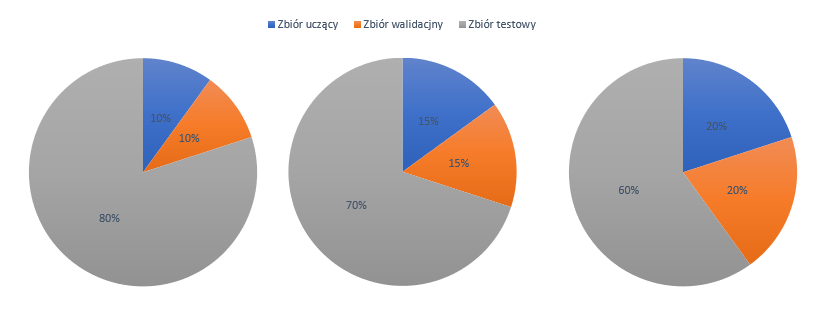
\includegraphics[height=5.5cm]{partials/images/machine_learning_process_1.png}
	\caption{Przykład podziału danych na zbiory treningowe, walidacyjne i testowe}
\label{Fig:MachineLearningProcess1}
\end{figure}

Najczęściej, podział na zbiory dokonuje się w proporcjach 70-80\% na trening, 10-15\% na walidację i 10-15\% na testy.
Jest to zależne od specyfiki problemu,
dlatego konieczne jest odpowiednie przygotowanie i zbadanie danych przed podjęciem decyzji.

Wybór modelu to proces, który zależy od rodzaju problemu (np. regresja, klasyfikacja, klasteryzacja)
oraz charakterystyki danych, gdzie najpopularniejsze modele to drzewa decyzyjne,
lasy losowe, maszyny wektorów nośnych (SVM), sieci neuronowe, k-najbliższych sąsiadów (k-NN)
i regresja liniowa/logistyczna. Trenowanie modelu to kolejny etap,
który polega na dostosowaniu parametrów modelu do danych treningowych,
w tym dostosowaniu hyperparametrów modelu (parametrów, które nie są uczone,
np. liczba warstw w sieci neuronowej) poprzez metodę walidacji krzyżowej lub inne techniki optymalizacji.

Ewaluacja obejmuje ocenę modelu za pomocą pewnych metryk,
takich jak dokładność, precyzja, recall, F1-score, błąd średniokwadratowy (MSE),
błąd absolutny (MAE), a także analizy wydajności modelu w przypadku klasyfikacji binarnej.
Optymalizacja modelu to kolejny etap, który obejmuje dalsze dostosowanie hyperparametrów,
wybór cech, które najbardziej wpływają na wynik modelu,
próby różnych architektur modelu oraz zastosowanie technik takich jak L1, L2, dropout,
które zapobiegają przeuczeniu modelu.

Implementacja modelu jest procesem, w którym wdrażany jest model w środowisku produkcyjnym.
Zakłada ona przeprowadzenie integracji z aplikacjami zewnętrznymi, tworzenie API serwujących dane,
zautomatyzoawanie decyzji, czy też śledzenie wydajności modelu w czasie rzeczywistym,
aby wykryć ewentualne pogorszenie jakości (drift danych) i regularne aktualizacje modelu.
Aktualizacja i utrzymanie modelu to kolejny etap,
który obejmuje regularne aktualizowanie modelu na podstawie nowych danych,
aby utrzymać jego dokładność i skuteczność, ciągłe monitorowanie,
aby zapewnić, że model działa zgodnie z oczekiwaniami i nie występują niepożądane zachowania.
Proces uczenia maszynowego jest iteracyjny i wymaga ciągłej interakcji między danymi,
modelem i wynikami, aby osiągnąć optymalne rezultaty.